\chapter{Results and Discussion}
\section{Thicknesses and densities of a-Si and SiO\texorpdfstring{$_{2}$}{2} thin films}\label{sec: results_thicknesses}
~\ref{fig: thz_substance} and~\ref{fig: thz_subs} show the XRR measurements of various a-Si films grown on glass substrates with varying thicknesses according to the quartz crystal microbalance (QCM) readings across different growth runs. From the graphs of the intensity the $2\theta$ range at which the detector can still detect the reflected x-rays generally ranges from \ang{0.3} to \ang{1.5}. The measured thicknesses of the a-Si film based on XRR are summarized in~\ref{tab: thickness_a-Si}, while for SiO$_2$ the results are summarized in~\ref{tab: thickness_SiO2}. No thickness data could be obtained from XRR for films which were thicker than \qty{1.52}{\kilo\meter} for a-Si and \qty{1.369}{\kilo\meter} for SiO$_2$. Linear regression of the measured thicknesses versus the QCM readings for a-Si as shown in~\ref{fig: thz_subs} yields the equation
\begin{equation} \label{eqn:aSi_thickness} 
    y = 167.82x + 2.749
\end{equation}
with $R^2 = 0.9999$, where $y$ is the measured XRR thickness in \unit{\nano\meter} and $x$ is the QCM reading in \unit{\kilo\meter}. Similarly, linear regression of the measured XRR thickness and the QCM values for SiO$_2$ as shown in~\ref{fig: thz_subs} yields the equation
\begin{equation} \label{eqn:SiO2_thickness} 
    y = 199.49x - 5.4845
\end{equation}
with $R^2 = 0.9937$. 

\begin{table}[tbp]
\centering
\begin{tabular}{ll}
\toprule
QCM (kA) & XRR (nm) \\
\midrule
0.035    & 6.9      \\
0.138    & 27.5     \\
0.104    & 21.1     \\
0.069    & 13.7     \\
1.52     & 257.7    \\
\bottomrule   
\end{tabular}
\caption{a-Si thickness}\label{tab: thickness_a-Si}
\end{table}

\begin{table}[tbp]
\centering
\begin{tabular}{ll}
\toprule
QCM (kA) & XRR (nm) \\
\midrule
1.05     & 204.3    \\
0.525    & 103.7    \\
0.884    & 162.9    \\
1.369    & 270.8    \\
\bottomrule
\end{tabular}
\caption{SiO2 thickness}\label{tab: thickness_SiO2}
\end{table}

The initial comparison of the QCM readings and the measured thicknesses during XRR indicate that the QCM readings during deposition generally underestimate the actual thicknesses of the films. However, the results of the regression analysis indicate that the QCM readings scale linearly with the actual thicknesses of the films as measured by XRR\@. The high $R^2$ values suggest that the QCM is a reliable tool for monitoring film thickness during deposition as long as the linear relationship is considered, and that the linear relationships obtained in this study can be used to calibrate the QCM readings for future depositions. The lower $R^2$ value in the regression for SiO$_2$ is attributed to the variation in the deposition rate during the growth of the SiO$_2$ films, which is caused by the difficulty in maintaining a stable deposition rate for SiO$_2$ due to its low thermal conductivity and tendency to sublime instead of melting into a uniform liquid pool during heating by the electron beam as is the case for other materials. \ref{fig: thz_subs} and~\ref{fig: thz_subs} show the source materials inside the crucibles for electron beam evaporation, with the a-Si source material melting uniformly while the SiO$_2$ source material shows localized heating and uneven melting.

\begin{figure}
	\centering
	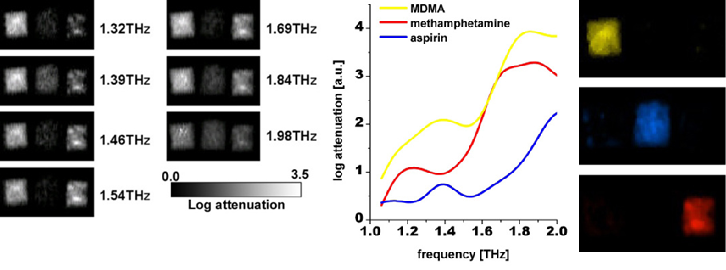
\includegraphics[width=0.85\textwidth]{figures/thz_subs.png}
	\caption[THz spectra of substances]{THz identification of MDMA, methamphetamine, and aspirin through a paper envelope. The substances are differentiated using their THz spectra}\label{fig: thz_subs}
\end{figure}

\section{Refractive index of a-Si thin films}\label{sec: results_index_Si}
\ref{fig: thz_subs} shows the UV-Vis transmittance spectra of a \qty{600}{\nano\meter} a-Si thin film deposited on a glass substrate together with the upper and lower envelopes as calculated using the Swanepoel method. The equations of the exponential function envelopes fitted to the extrema points listed in \ref{tab: thickness_SiO2} are
\begin{equation} \label{eqn:aSi_upper_env} 
    y = 80.612419+1200883000e^{-x/89.819343}-1200749000e^{-x/89.821415}
\end{equation}
for the maxima with $R^2 = 0.9969$ and 
\begin{equation} \label{eqn:aSi_lower_env} 
    y = 45.9178758+31602801200e^{-x/64.3969697}-31601554900e^{-x/64.3973202}
\end{equation}
for the minima with $R^2 = 1$. The equation for the refractive index of the a-Si thin film according to Sellmeier's equation from the data points of the refractive indices obtained from Swanepoel's method is
\begin{equation} \label{eqn:aSi_sellmeier} 
    n^2 = 14.84529+\frac{\num{7.06709e12}\lambda^2}{\lambda^2+\num{2.12449e18}}+\frac{-10.41841\lambda^2}{\lambda^2+190469.027}
\end{equation}
. The average thickness of the a-Si thin film according to the Swanepoel method is \qty{653}{\nano\meter}.



\section{Refractive index of SiO\texorpdfstring{$_{2}$}{2} thin films}\label{sec: results_index_SiO2}
